\documentclass[midd]{thesis}

\usepackage{graphicx}
\usepackage{times}

\bibliographystyle{plain}

\title {Can You Guess Where I Am?\\ Geolocating Tweets with Text Classification}

\author {Will Potter}
\adviser {Professor David Kauchak}

\begin{document}

\maketitle

\begin{abstract}
With massive amounts of textual data being shared on the web, through blogs, social media, websites pictures, the opportunity for extracting relevant metadata is expanding, including geographic information. While GPS-enabled devices are becoming more popular, many people with mobile phones would prefer to not share their locations with applications and companies. Additionally, IP geolocation, often isn't available or completely accurate.  This study trained traditional text classifiers on geotagged Twitter data (Tweets) using the text statuses as the features and the geographic location as labels in order to predict the location of tweets based exclusively on their text. The dataset contained 144,856 English-language tweets sent from the 50 United States and the District of Columbia. Training on randomly selected sets of roughly 16,000 tweets, the best classification methods yielded just over a 2\% accuracy boost when compared with choosing the most frequently occuring label in the training set. While the practical applications of replicating this experiment in commericial environments are small, it shows that a larger dataset might yield more promising results.


\end{abstract}

\begin{acknowledgements}
% 
\end{acknowledgements}

\contentspage
\tablelistpage
\figurelistpage

\normalspacing \setcounter{page}{1} \pagenumbering{arabic}

\chapter{Introduction}

\section{Classification of Social Media}

The rapid growth of social media in the past 10 years has shown that people are living their lives increasingly more through the internet and are sharing more information with more people than ever before in history. At the end of 2013, Facebook had 1.23 billion monthly active users \cite{facebookabout} and Twitter had 241 million monthly active users \cite{twitterabout} -- and those are just the largest two networks. People are sharing content online through Pinterest, Foursquare, Tumblr and many other sites. Yet while the number of social media users has expanded, much about their behavior is still difficult to determine.

As people share information, companies analyze user information to help data monetization efforts, such as advertising. A local fast food restaurant in Burlington, Vermont might like to target Twitter users who not only like fast food, but also live within a certain radius of the restaurant. Increased targeting filters allow companies to reduce the amount of total advertising dollars needed for user engagement. 

While the principle is simple, analyzing this data becomes increasingly more complex as the size of the data increases--Twitter, alone, manages 500 million tweets per day. Deriving useful conclusions from such a large dataset requires an intricate knowledge of the data before effective analysis can be applied.

\section{Smartphones and Geotagging}
In addition to the growth of social media, the world has seen the adoption of the Internet connected smartphones. Business Insider found that 22\% of the global population owned a smartphone at the end of 2013\cite{businessinsider}. People are sharing more and doing so wherever they go. More than ever, phone users have the ability to share their GPS location apps and social media sites. This opportunity gave way to the creation of Foursquare, a geographic social network that allows users to broadcast their location to other users and local businesses. As Foursquare refined their idea, Facebook and Twitter soon followed with location-sharing services inside their mobile apps. Even though these features are now a part of many social media apps, location sharing has not seen widespread adoption. Estimates show that roughly 2\% of tweets sent at any given moment contain geographic information.\cite{heartbeat:leetaru}

Geotagging is particularly useful for advertising, as well as business intelligence. Twitter, while an incomplete sample of the population, can serve as a tracking agent for businesses. While the requirement that people ``opt-in" to sharing their location may be a bias in the data, companies still may use geotagged tweets as a random sample of all social media users when running analytics to generalize conclusions across an entire user base. For example, McDonald's might like to show an advertisement for someone who works immediately next to one, but has never tweeted or checked-in at a their restaurant. A user's proximity to a certain business makes them a more appealing ad target, which in turn provides a premium experience for advertisers to use. A McDonald's or Target would greatly prefer to target people who live nearby or pass through town rather than simply targeting based on a user's interests, tweets or follows.

Given that Twitter only records a definitive location for 20\% of their tweets, they lose out on location information for the rest of the almost 80\% of their users. If a social network were to mandate location sharing, the company would be perceived as grossly violating individual privacy rights and would almost certainly lose many users, thus decreasing the underlying value of their service. Even if the locations were automatically collected and kept private, smartphone manufacturers, like Apple, could disable GPS-use on their phones to protect users. If a social network had some way at guessing the location of a user based purely based on the content of their update (i.e. a tweet's body or a Facebook status' text), they would be able to provide a superior analytic experience without storing the exact geographic coordinates of a user. Additionally, the network would be using information that the user implicitly consents to public sharing (by nature of using a social network in the first place).

This thesis looks to examine the possibility of determining a user's location at the point of sharing (or close to the point of sharing) based on text classification and clustering around the content of their update. Specifically, it will use a set of geotagged tweets acquired from Twitter's public API as training data for running a series of machine learning algorithms on the text of tweets. By training on already geo-tagged tweets, which appear to have virtually the same content as non-geotagged tweets, anyone could later predict locations for the remaining 80\% of tweets. This thesis will focus on English language tweets, as tagged by the Twitter API, but the methods could hopefully carry over to other languages as well.

While initial efforts target exclusively the body text of tweets, incorporating user information into classification should improve results. Accounting for the location of other tweets by the same user and the user's stated location in their settings should help influence the classification result especially if classification efforts narrowed it down to a small number of places. Additionally, using the time as a feature should help, as most people operate in regular cycles (daytime at a place of work or school, and nighttime at home).

As many words bear certain significance to a particular geographic location, it can be expected that different types of words will have an effect on predicting the location of a tweet. At the simplest level, referring to place names, such as New York, Boston, or San Francisco, can be expected to have a correlation to the location of the tweeter. It may relate to something in the past (``Just got back from New York City...great weekend."), present (``I'm at New York Hilton Midtown - @hiltonhotels (New York, NY)"), future (``3 hours to go until New York will be calling! \#fashion \#opportunity \#career"). The user may not even be planning to go to the place, but rather just is referencing the place (``If only New York wasn't so far away").

Additionally, the use of neighboorhoods or other place names may indicate a geographic location. Tweets like ``I ❤️ SNOW \#nyc @ Hell's Kitchen - NYC" refer to the Hell's Kitchen neighboorhood in NYC but tweets refer to other cultural features, like the TV show ``Hell's Kitchen": ``Literally can't get enough of @GordonRamsay `a Hell's Kitchen' - absolute stormer of a show, can't wait for the new series".

Finally, the presence of particular words, like ``frappe" and ``milkshake" may indicate if someone is in a particular location. Tweets with ``frappe" are less popular and appear in the Northeast mainly, while ``milkshake" appears more frequently and across a greater geographic area.

Using a fair degree of knowledge about the use cases of Twitter,  can hope to see some success in analyzing a tweet's textual body to infer the location of a user.

With some degree of knowledge regarding Twitter's use cases, designing a text classification model should yield positive and productive results for determining the location of tweets based exclusively on their text bodies.

\chapter{Related Work}

Founded in 2007, Twitter is a relatively new platform. Like most parts of the high tech sector, it has changed and evolved rapidly, starting as a text messaging based app that ultimately transitioned to mobile and web application based network. As Twitter has grown, it has seen increased interest from academics for its representation of realtime human dialogue and movement. Kwak et al. \cite{kwak2010twitter} found that Twitter had transformed into a hybrid social network and news medium. Given the low user reciprocity around sharing as well as the high average retweet count for an average tweet, it resembles a crowd-sourced news network almost as much as a person-to-person network.

Building on the crowd sourced news network description, researchers created systems that record and plot geo-tagged tweets and photos on a map, to show a heatmap effect regarding Twitter activity at any given moment. \cite{nakaji2012visualization} \cite{yanai2012world}

Kinsella et al. \cite{kinsella2011m} started to consider the idea of geotagging tweets by comparing it with several other forms of geotagging. Using a baseline constructed from a tweet's GPS coordinates, they considered geotagging based on a user's self reported location as well as a tweets content. They then compared this to the majority label in a given dataset.

Twitter's ability to analyze realtime communication across the globe has allured researchers to consider various questions, especially where users are when they tweet. Despite Twitter's included GPS coordinates, others have tried to extract location information from a tweets content. Using a highly specific dataset consisiting of Twitter users with over 1000 tweets and a listed profile location in the continental United States, Cheng et al. \cite{cheng2010you} were able to achieve an accuracy rate of 51\% when classifiying user's locations. Initially, they identified local words, such as ``tortilla'', ``redsox'' or ``canyon''. By combining the geographic centers of each of these words, they probabalistically determined a new centroid for a likely area of the tweet in question. 

Roller et al. \cite{roller2012supervised} compared the text from tweets to definitive, fact-heavy text from Wikipedia downloaded. Their experiments could correctly geolocate the tweets with 161km of its true location 90\% of the time. By using a k-dimensional tree, they recursively broke up the geographic grid to best identify which node fit the testing data. Training data included the wikipedia data containing many place names and toponyms. They then compared a tweet to the wikipedia text, knowing that placenames included in tweets would correlate to a particular document from wikipedia often.

Additionally, the tweet corpus has been analyzed to search for spatiotemporal anomalies, such as natural disasters or societal events, like riots or protests through clustering tweets across time. Their study produced relevant visualizations that would accurately overlay the type of disturbance on a map, based on the trending terms used in tweets. \cite{thom2012spatiotemporal} 


\chapter{Data and Preprocessing}
\section{Data}

Data was collected from the Twitter API by querying their streaming API for all tweets with an attached pair of geographic coordinates or an attached geofenced region. Tweets with a region attached were assigned the midpoint of the region. 

The dataset is comprised of 144,546 tweets with 84,860 unique users tweeting on February 13, 2014. This sample represents all geotagged, English-language tweets collected over random time intervals during the above period. Additionally, all tweets were sent from locations in the United States. Collection from the Twitter API occasionally times out, leaving gaps where tweets were not collected. As Twitter publishes approximately 500 million tweets per day\cite{twitterabout}, this dataset represents a small minority of tweets. While small, it still provides a nice starting set useful for running experiments on a personal computer without significant performance issues.

Geographically, all tweets were sent from within the 50 United States, as well as Washington D.C. Overseas territories and minor outyling islands were not included. All 50 States (and D.C.) were represented all 50 states and Washington D.C., however only 2570 of 3,144 counties or county equivalents were represented. Some counties, like New York County (Manhattan), represented with 1,256 tweets (0.8\% of the dataset), or Los Angeles County, represented with 3,879 tweets (2.7\%), held disproportionately high numbers of tweets as they both have disproportionately large populations for a county.

\begin{figure}
\centering
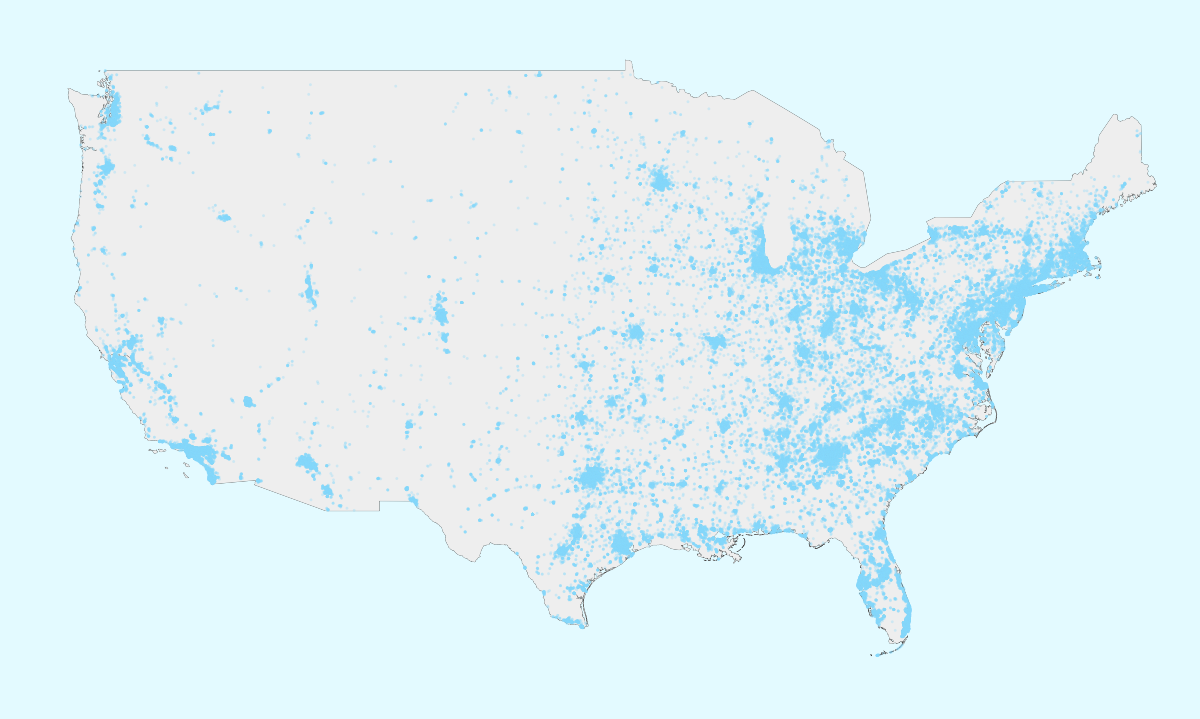
\includegraphics[width=0.85\textwidth]{full_country_map.png}
\caption{All Tweets from the study's dataset in the Lower 48 United States.}
\label{fig:tweetmap}
\end{figure}

In addition to Twitter data, 122,816 geotagged Wikipedia articles were used to provide another training corpus. Given the large number of place specific terms, Wikipedia articles could be effective at ``teaching'' a model the textual representation of a particular location. For example, the article on the Boston Financial District contains ``street'', ``headquarters'', ``financial'', ``bank'' and ``boston'' as the 5 most used words, after stopwords are removed.

Wikipedia titles were acquired along with their geographic coordinates through dbpedia.org, and then downloaded through the raw Wikipedia API.


\section{Preprocessing}
Tweets tend to be informal and are filled with insignificant, popular words (``the", ``I", ``a") as well as a range of misspellings. In addition, tweets contain links and usernames that don't necessarily have a strong correlation to one's location. For this reason, simply counting each word as a feature is a naïve approach that introduces an unwanted amount of noise to classification experiments.

In addition to testing the effects of different classifiers, an experiment was constructed to test the effects of preprocessing the data. Experiments without preprocessing enabled used the raw content from the tweet, with all original characters left untouched. Preprocessing, however, heavily modified the body of the tweet by stripping capitalization, symbols, links, usernames and common English words, known as stopwords. By removing capitalization, the total number of features in the training model is reduced. This reduction in the total number of words should decrease the chance that valuable features are outweighed by meaningless features. Furthermore, removing symbols, links and usernames should decrease the total number of features in the classifier, giving a more accurate representation of what people mean, rather than the literal text representation. While some usernames, like ``@bostonglobe'', do contain valuable information, most appeared to lack any relevant geographic information in their name. Hashtags (i.e. ``\#bostonstrong''), often contain geographic information, however, pound symbols were removed to ensure ``\#nyc'' and ``nyc'' would resolve to the same feature. Table~\ref{table:preprocessing} shows examples of input and output to the preprocessing method. While all features referring to a geographic entity are not reduced to the same feature, the preprocessing method reduces the 13 sample features with preprocessed features storing counts more.


\begin{table}
\label{table:preprocessing}
\caption{Examples of the effect of preprocessing on expressions.}
\centering 
  \begin{tabular}{| c | c |}
  \hline
  Before & After \\
  \hline
  ``Boston'' & ``boston'' \\
  ``(Boston, MA)'' & ``boston ma'' \\
  ``Boston's'' & ``bostons'' \\
  ``Boston?'' & ``boston'' \\
  ``Boston, MA'' & ``boston ma'' \\
  ``\#boston'' & ``boston'' \\
  ``\#bostonma'' & ``bostonma'' \\
  ``@bostonhockey'' & ``'' \\
  ``We are Boston!'' & ``boston'' \\
  \hline  
  \end{tabular}
\end{table}

\section{Labels}
To achieve the best accuracy, labels should take advantage of natural divisions between the population. In theory, people living in the same community will generally refer to the same places, whether that community is a state, metropolitan area, town or a neighborhood. Unfortunately, running experiments on tweets labeled by their town or neighborhood is difficult on a personal computer.

\subsection{Geographic Grid Regions}
In running experiments, labels are derived from the geographic coordinates of a tweet. As the labels run across a wide range of real numbers in 2 dimensions, effectively labeling the training features is a non-trivial process. The easiest way to label tweets is to break up the geographic into regions of equal latitude and longitude intervals. This, however, ignores cultural boundaries and dense areas. A 1-degree x 1-degree ``bucket" in Montana has a smaller and more homogenous population with fewer places. However, the ``bucket" including New York City would have many more people, places and material and determining if a tweet originated there would be difficult. Given the inequality of area as latitudes change, this can be expected to behave differently for regions on the equator when compared with polar regions. While most of the world's population and tweets do not originate from the extreme poles, northern/southern regions will be broken into smaller buckets than central areas.

\begin{figure}
\centering
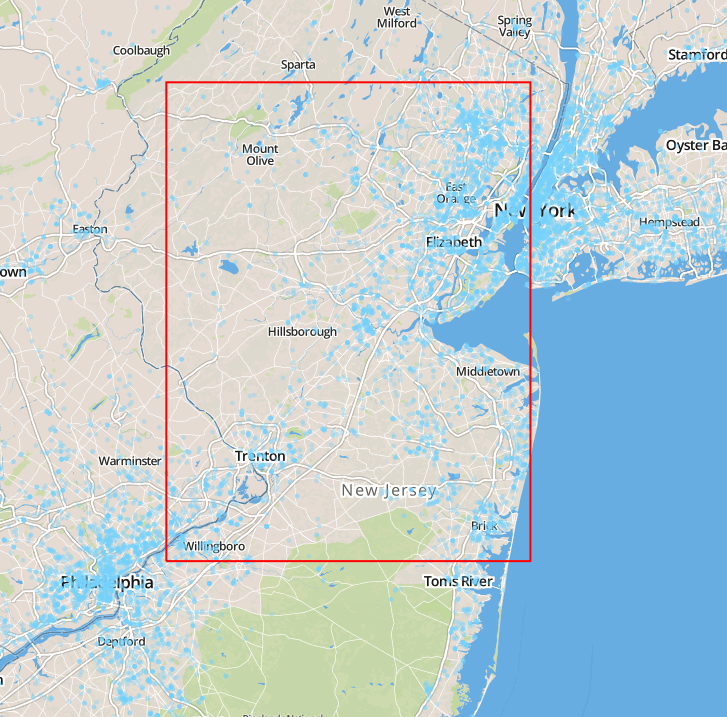
\includegraphics[width=0.75\textwidth]{grid_zone.png}
\caption{A one degree by one degree zone labeling bucket.}
\label{fig:grid_zone}
\end{figure}

\begin{figure}
\centering
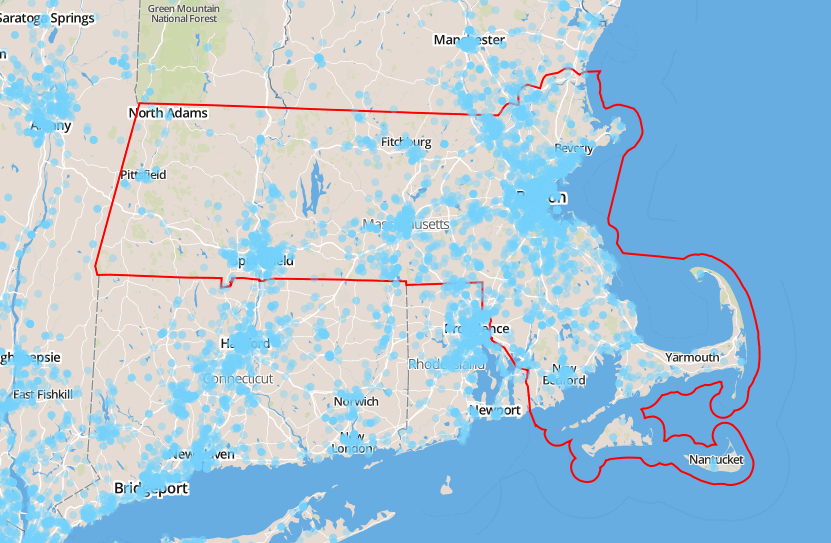
\includegraphics[width=0.75\textwidth]{state_zone.png}
\caption{A labeling zone for Massachusetts.}
\label{fig:state_zone}
\end{figure}

\subsection{Political Boundaries}
As latitude and longitude lines often run across political boundaries, the grid-based approach is likely to include training data from the same population in two separate examples. For example, Manhattan is bisected by two separate buckets with the 1x1 degree scale with Trenton, NJ and parts of the Philadelphia suburbs included in the Western bucket and parts of Long Island falling into the Eastern bucket. See Figure~\ref{fig:grid_zone}. 

Tweets were labeled with two separate resolutions for experiements: state and county. Each tweet was given a numeric FIPS (Federal Information Processing Standard) label corresponding to a state. Figure~\ref{fig:state_zone} shows a sample zone, where the metropolitan areas around Boston, Worcester and Springfield are largely captured in the same label. While New Hampshire and Rhode Island may pick up on some of the population that either lives, works or visits the Boston metropolitan area, most of the community is encompassed.

\begin{figure}
\centering
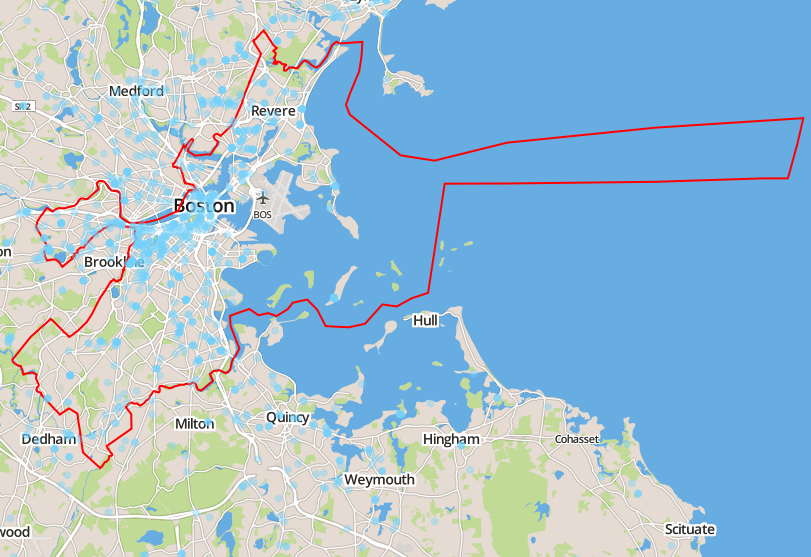
\includegraphics[width=0.75\textwidth]{county_zone.png}
\caption{A labeling zone for Suffolk County, Massachusetts.}
\label{fig:county_zone}
\end{figure}

This study does not label tweets on a Metropolitan/Micropolitan/Rural scale, however future studies should consider that these boundaries may segment people more naturally than state and county lines.

\chapter{Experimental Methods}

\section{Setup}
Taking the dataset of geotagged tweets, this study structures its experiments as a classification problem. The tweets in question are already geotagged, thus providing a definitive definition of where they were written. With this in mind, the goal is to predict the geographic coordinates of tweets without included geodata.

\section{Scope}
While the dataset only comprises English language tweets, tweets are saved from around the world. Given the lack of English speakers in many regions of the world, it could be problematic to label the entire world, as a region in Africa will have substantially fewer training examples than a region in Fairfield County, CT would have. Experiments will examine the continental US separately in addition to attempting worldwide classification.



\section{Data Training and Testing Protocols}

\subsection{Randomness and Cross Validation}
Due to performance limitations,  experiments ran with 20000 examples. From the 144,456 US tweet corpus, tweets are randomly selected for each experiment. All models then run on the same random, 20000-example sample to avoid variation that might stem from pulling drastically different sets from the complete corpus.

Additionally, to account for variation that might occur within 1 experiment, experiments are performed at least 15 times. Given our performance limits and the 20,000 tweet limit, we're able to select a new set of 20,000 tweets to train on. As one of our benchmarks for performance is accuracy relative to the strategy of choosing the majority label and each subset has a slightly different majority label, we calculate performance relative to  the majority strategy. Accuracy is defined in Equation~\ref{eqn:accuracy}, and improvement is defined in Equation~\ref{eqn:improvement}

\begin{equation}
\label{eqn:accuracy}
accuracy_{test}=\frac{examples_{correct}}{examples_{total}}
\end{equation}

\begin{equation}
\label{eqn:improvement}
improvement=accuracy_{test} - \frac{examples_{majority}}{examples_{total}}
\end{equation}

Within each fold, the data is split into 80\% training and 20\% testing.

\section{Supervised Learning Models}
\subsection{K-Nearest Neighbor}

K-Nearest Neighbor classification examines a set of training examples and using their features and internally stores them on an n-dimensional space. In our case, features are words or n-grams included in the body text of tweets. Then with a test example, the model identifies the K-nearest examples and chooses the majority label.

In order to mitigate the risk of insignificant terms weighting the distance metrics for each example, a term frequency-inverse document frequency (TF-IDF) vectorizer can be used instead of a  normal count vector. TF-IDF vectors weight words that appear the most in a given document but negatively weight words that appear in many documents.


\subsection{Naive Bayes}

Using the Naive Bayes model for text classification introduces another method to improve accuracy. While an effective model, our data should be preprocessed to ignore many of the random noise words included in most tweets. With each ineffective term in the training set, the overall effectiveness of Naive Bayes decreases. When training on a toponym heavy dataset like Wikipedia, Naive Bayes can be quite effective.

\subsubsection{Multinomial Naive Bayes}

The simpler of the two classifiers, Multinomial Naive Bayes classifier, examples are given a label based on the likelihood that each of their features has a certain label. As shown in Equation~\ref{eqn:multinomialNaiveBayes}, the model examines both the probability that a document has a specific label, as well as the probability that each word is used in that label. The label chosen is the one with the highest probability.

\begin{equation}
\label{eqn:multinomialNaiveBayes}
max(p(f_1, \dots, f_n \vert L) )= max(p(L) \prod_{i=1}^n (L|f_i))
\end{equation}

\subsubsection{Bernoulli Naive Bayes}

Unlike Multinomial Naive Bayes, Bernoulli Naive Bayes (BNB) doesn't care about word counts and relative probabilities. Rather BNB merely looks for the presence or absence of a particular feature. Bernoulli Naive Bayes doesn't account for one word appearing many more times than another word.


\chapter{Experimental Results and Examples}


\section{Results}
\subsection{Classification}


In general, classifying locations based on the text of a tweet proved to be incredibly difficult. Given that many tweets lack any meaningful location information. Out of 10 randomly pulled tweets, only one contained a reference to a location. The tweet, ``If Pittsburgh wins this...'', didn't even overtly reference the author's location. While the author may have been a Pittsburgh sports fan, there is a good chance that they were supporting the other team as well. As such, results were difficult to gauge and success came in small amounts. Improving accuracy by 1 or 2 percent above ``Majority Strategy'' was good, given that only 1 in 100 tweets might contain useful location information. General accuracy for the final methods can be found in Table~\ref{table:finalResults}.

\begin{table}
\label{table:finalResults}
\caption{Improvement upon choosing the majority label. \textbf{Bold} results are significant at a 5\% confidence interval and \textit{italic} results are significant at a 10\% confidence interval.\newline }
\centering 
  \begin{tabular}{| c | c | c | c | c  | c |}
  \hline      
Classifier & Preprocessing & Labeling & Test Improvement & P-Value \\
  \hline                 
Multinomial NB & No Preprocess & State  & \textbf{2.196\%} & 6.93E-41 \\
Multinomial NB & Preprocess & State  & \textbf{2.109\%} & 5.39E-38 \\
Bernoulli NB & No Preprocess & State  & \textbf{1.442\%} & 7.03E-36 \\
Bernoulli NB & Preprocess & State  & \textbf{1.422\%} & 2.42E-38 \\
Multinomial NB & Preprocess & County & \textbf{0.427\%} & 3.69E-27 \\
Bernoulli NB & Preprocess & County & \textbf{0.416\%} & 1.29E-30 \\
KNN-1000 & No Preprocess & State  & \textbf{0.231\%} & 0.0039 \\
KNN-2000 & No Preprocess & State &  \textbf{0.183\%} & 0.0212 \\
Multinomial NB & No Preprocess & County & \textbf{0.165\%} & 6.77E-17 \\
Bernoulli NB & No Preprocess & County & \textbf{0.156\%} & 4.00E-18 \\
KNN-1000 & Preprocess & State & \textbf{0.120\%} & 0.0332 \\
KNN-2000 & Preprocess & State & 0.081\% & 0.1178 \\
KNN-2000 & No Preprocess & County & -0.001\% & 0.1813 \\
KNN-1000 & Preprocess & County & \textit{-0.009\%} & 0.0771 \\
KNN-1000 & No Preprocess & County & \textit{-0.024\%} & 0.0707 \\
KNN-100 & No Preprocess & State & \textbf{-0.156\%} & 0.0207 \\
KNN-50 & No Preprocess & State & \textbf{-0.534\%} & 2.65E-09 \\
KNN-100 & Preprocess & State & \textbf{-0.788\%} & 1.61E-10 \\
KNN-100 & No Preprocess & County & \textbf{-0.809\%} & 1.06E-26 \\
KNN-100 & Preprocess & County & \textbf{-0.880\%} & 8.16E-20 \\
KNN-50 & No Preprocess & County & \textbf{-1.173\%} & 1.37E-43 \\
KNN-50 & Preprocess & State & \textbf{-1.180\%} & 5.70E-21 \\
KNN-50 & Preprocess & County & \textbf{-1.214\%} & 1.67E-30 \\  
\hline  
  \end{tabular}
\end{table}


\subsection{KNN/Grid Labeling Results}
As shown in the table below, K-Nearest Neighbor increases accuracy with an increase in clusters. With both labeling schemes, they don't appear to improve beyond K values of 128. K values of 128 appear to slightly dominate choosing exclusively the majority label.

\subsection{Naive Bayes}

Using both Naive Bayes variants yielded better results over the KNN classifier. Given the sparsity of the Twitter data, it is possible that the nearest neighbors were chosen based on words the tweets shared. Given the short timeframe while the Tweets were collected, its possible that temporal events affected the nearest neighbors of the tweets. Tweets were collected during Valentines day and the word ``valentine'' appears in the top 100 words of the US-tweets dataset.

\subsection{State/County Boundary Results}


\begin{table}
\label{fig:labelingResults}
\caption{Difference in percent improvement over randomly guessing the majority label between State and County labels for certain classifiers. \textbf{Bold} results are significant with a 5\% confidence interval. $n=60$ for each classifier. Significance was tested using a 2-tailed, paired T-test.\newline }

\centering 
  \begin{tabular}{| c | c | c |}
  \hline      
  Classifier & Test Improvement & P-Value \\
  \hline
\textbf{Bernoulli NB No Preprocessing} &\textbf{ 1.285\% }& \textbf{ 3.80E-32 }\\
\textbf{Bernoulli NB Preprocessing} &\textbf{ 1.006\% }& \textbf{ 6.35E-30 }\\
\textbf{Multinomial NB No Preprocessing} &\textbf{ 2.032\% }& \textbf{ 2.19E-38 }\\
\textbf{Multinomial NB Preprocessing} &\textbf{ 1.682\% }& \textbf{ 2.87E-31 }\\
\textbf{KNN-50 No Preprocessing}&\textbf{ 0.639\% }& \textbf{ 4.00E-10 }\\
KNN-50 Preprocessing & 0.033\% & 0.6877 \\
\textbf{KNN-100 No Preprocessing} &\textbf{ 0.652\% }& \textbf{ 3.59E-11 }\\
KNN-100 Preprocessing & 0.092\% & 0.3773 \\
\textbf{KNN-1000 No Preprocessing} &\textbf{ 0.255\% }& \textbf{ 0.0022 }\\
\textbf{KNN-1000 Preprocessing} &\textbf{ 0.129\% }& \textbf{ 0.0209 }\\
\textbf{KNN-2000 No Preprocessing} &\textbf{ 0.184\% }& \textbf{ 0.0204 }\\
KNN-2000 Preprocessing & 0.081\% & 0.1178 \\
  \hline  
  \end{tabular}
\end{table}



When using states and counties as labels, states tended to be more effective at predicting location. Regardless of the classifier used, state labels could be predicted more effectively than county labels, however some classifiers lacked statistical significance between using difference labeling schemes. Given that some of the counties had very few tweets, they most likely lacked sufficient training featurest to train a meaningful classifier. States, however, had many more tweets per label and more meaningful classifiers could be generated.

\subsection{Preprocessing}


\begin{table}
\label{fig:preprocessingResults}
\caption{Difference between Preprocessing and Non-preprocessing in percent improvement over randomly guessing the majority label. \textbf{Bold} results are significant with a 5\% confidence interval. $n=60$ for each classifier. Significance was tested using a 2-tailed, paired T-test.\newline}
\centering 
  \begin{tabular}{| c | c | c |}
  \hline      
  Classifier & Test Improvement & P-Value \\
  \hline                 
Bernoulli NB State & -0.0199\% & 0.746 \\
\textbf{Bernoulli NB County} & \textbf{0.2592\%} & \textbf{2.07E-16} \\
Multinomial NB State & -0.0874\% & 0.346 \\
\textbf{Multinomial NB County} & \textbf{0.2629\%} & \textbf{2.30E-14} \\
\textbf{KNN-50 State} & \textbf{-0.6461\%} & \textbf{1.26E-07} \\
KNN-50 County & -0.0404\% & 0.530 \\
\textbf{KNN-100 State} & \textbf{-0.6312\%} & \textbf{3.76E-06} \\
KNN-100 County & -0.0713\% & 0.369 \\
KNN-1000 State & -0.1107\% & 0.259 \\
KNN-1000 County & 0.0150\% & 0.289 \\
KNN-2000 State & -0.1017\% & 0.269 \\
KNN-2000 County & 1.23E-05 & 0.181 \\
  \hline  
  \end{tabular}
\end{table}



Curiously enough, preprocessing did not have a significant effect on accuracy. Studies are still ongoing to determine the significance of preprocessing.




\section{Examples}

\chapter{Conclusion}




\appendix
\chapter{List of Stopwords}
 ``a'', ``able'', ``about'', ``above'', ``abst'', ``accordance'', ``according'', ``accordingly'', ``across'', ``act'', ``actually'', ``added'', ``adj'', ``affected'', ``affecting'', ``affects'', ``after'', ``afterwards'', ``again'', ``against'', ``ah'', ``all'', ``almost'', ``alone'', ``along'', ``already'', ``also'', ``although'', ``always'', ``am'', ``among'', ``amongst'', ``an'', ``and'', ``announce'', ``another'', ``any'', ``anybody'', ``anyhow'', ``anymore'', ``anyone'', ``anything'', ``anyway'', ``anyways'', ``anywhere'', ``apparently'', ``approximately'', ``are'', ``aren'', ``arent'', ``arise'', ``around'', ``as'', ``aside'', ``ask'', ``asking'', ``at'', ``auth'', ``available'', ``away'', ``awfully'', ``b'', ``back'', ``be'', ``became'', ``because'', ``become'', ``becomes'', ``becoming'', ``been'', ``before'', ``beforehand'', ``begin'', ``beginning'', ``beginnings'', ``begins'', ``behind'', ``being'', ``believe'', ``below'', ``beside'', ``besides'', ``between'', ``beyond'', ``biol'', ``both'', ``brief'', ``briefly'', ``but'', ``by'', ``c'', ``ca'', ``came'', ``can'', ``cannot'', ``can't'', ``cause'', ``causes'', ``certain'', ``certainly'', ``co'', ``com'', ``come'', ``comes'', ``contain'', ``containing'', ``contains'', ``could'', ``couldnt'', ``d'', ``date'', ``did'', ``didn't'', ``different'', ``do'', ``does'', ``doesn't'', ``doing'', ``done'', ``don't'', ``down'', ``downwards'', ``due'', ``during'', ``e'', ``each'', ``ed'', ``edu'', ``effect'', ``eg'', ``eight'', ``eighty'', ``either'', ``else'', ``elsewhere'', ``end'', ``ending'', ``enough'', ``especially'', ``et'', ``et-al'', ``etc'', ``even'', ``ever'', ``every'', ``everybody'', ``everyone'', ``everything'', ``everywhere'', ``ex'', ``except'', ``f'', ``far'', ``few'', ``ff'', ``fifth'', ``first'', ``five'', ``fix'', ``followed'', ``following'', ``follows'', ``for'', ``former'', ``formerly'', ``forth'', ``found'', ``four'', ``from'', ``further'', ``furthermore'', ``g'', ``gave'', ``get'', ``gets'', ``getting'', ``give'', ``given'', ``gives'', ``giving'', ``go'', ``goes'', ``gone'', ``got'', ``gotten'', ``h'', ``had'', ``happens'', ``hardly'', ``has'', ``hasn't'', ``have'', ``haven't'', ``having'', ``he'', ``hed'', ``hence'', ``her'', ``here'', ``hereafter'', ``hereby'', ``herein'', ``heres'', ``hereupon'', ``hers'', ``herself'', ``hes'', ``hi'', ``hid'', ``him'', ``himself'', ``his'', ``hither'', ``home'', ``how'', ``howbeit'', ``however'', ``hundred'', ``i'', ``id'', ``ie'', ``if'', ``i'll'', ``im'', ``immediate'', ``immediately'', ``importance'', ``important'', ``in'', ``inc'', ``indeed'', ``index'', ``information'', ``instead'', ``into'', ``invention'', ``inward'', ``is'', ``isn't'', ``itd'', ``it'll'', ``its'', ``itself'', ``i've'', ``j'', ``just'', ``k'', ``keep'', ``keeps'', ``kept'', ``kg'', ``km'', ``know'', ``known'', ``knows'', ``l'', ``largely'', ``last'', ``lately'', ``later'', ``latter'', ``latterly'', ``least'', ``less'', ``lest'', ``let'', ``lets'', ``like'', ``liked'', ``likely'', ``line'', ``little'', ``i'll'', ``look'', ``looking'', ``looks'', ``ltd'', ``m'', ``made'', ``mainly'', ``make'', ``makes'', ``many'', ``may'', ``maybe'', ``me'', ``mean'', ``means'', ``meantime'', ``meanwhile'', ``merely'', ``mg'', ``might'', ``million'', ``miss'', ``ml'', ``more'', ``moreover'', ``most'', ``mostly'', ``mr'', ``mrs'', ``much'', ``mug'', ``must'', ``my'', ``myself'', ``n'', ``na'', ``name'', ``namely'', ``nay'', ``nd'', ``near'', ``nearly'', ``necessarily'', ``necessary'', ``need'', ``needs'', ``neither'', ``never'', ``nevertheless'', ``next'', ``nine'', ``ninety'', ``no'', ``nobody'', ``non'', ``none'', ``nonetheless'', ``noone'', ``nor'', ``normally'', ``nos'', ``not'', ``noted'', ``nothing'', ``now'', ``nowhere'', ``o'', ``obtain'', ``obtained'', ``obviously'', ``of'', ``off'', ``often'', ``oh'', ``ok'', ``okay'', ``old'', ``omitted'', ``on'', ``once'', ``one'', ``ones'', ``only'', ``onto'', ``or'', ``ord'', ``other'', ``others'', ``otherwise'', ``ought'', ``our'', ``ours'', ``ourselves'', ``out'', ``outside'', ``over'', ``overall'', ``owing'', ``own'', ``p'', ``page'', ``pages'', ``part'', ``particular'', ``particularly'', ``past'', ``per'', ``perhaps'', ``placed'', ``please'', ``plus'', ``poorly'', ``possible'', ``possibly'', ``potentially'', ``pp'', ``predominantly'', ``present'', ``previously'', ``primarily'', ``probably'', ``promptly'', ``proud'', ``provides'', ``put'', ``q'', ``que'', ``quickly'', ``quite'', ``qv'', ``r'', ``ran'', ``rather'', ``rd'', ``re'', ``readily'', ``really'', ``recent'', ``recently'', ``ref'', ``refs'', ``regarding'', ``regardless'', ``regards'', ``related'', ``relatively'', ``research'', ``respectively'', ``resulted'', ``resulting'', ``results'', ``right'', ``run'', ``s'', ``said'', ``same'', ``saw'', ``say'', ``saying'', ``says'', ``sec'', ``section'', ``see'', ``seeing'', ``seem'', ``seemed'', ``seeming'', ``seems'', ``seen'', ``self'', ``selves'', ``sent'', ``seven'', ``several'', ``shall'', ``she'', ``shed'', ``she'll'', ``shes'', ``should'', ``shouldn't'', ``show'', ``showed'', ``shown'', ``showns'', ``shows'', ``significant'', ``significantly'', ``similar'', ``similarly'', ``since'', ``six'', ``slightly'', ``so'', ``some'', ``somebody'', ``somehow'', ``someone'', ``somethan'', ``something'', ``sometime'', ``sometimes'', ``somewhat'', ``somewhere'', ``soon'', ``sorry'', ``specifically'', ``specified'', ``specify'', ``specifying'', ``still'', ``stop'', ``strongly'', ``sub'', ``substantially'', ``successfully'', ``such'', ``sufficiently'', ``suggest'', ``sup'', ``sure'', ``the'', ``to'', ``too'', ``with'', ``was'', ``which'', ``that'', ``it'', ``this'', ``within'', ``include'', ``area'', ``000'', ``1'', ``2'', ``3'', ``4'', ``5'', ``6'', ``7'', ``8'', ``9'', ``0'', ``were'', ``we'', ``their'', ``there''

\chapter{Tweets by State}

  \begin{tabular}{| c | c || c | c || c | c |}
  \hline
\textbf{State} & \textbf{Total Tweets} & \textbf{State} & \textbf{Total Tweets} & \textbf{State} & \textbf{Total Tweets} \\
\hline
AL & 3422 & KY & 2445 & ND & 282 \\
AK & 203 & LA & 2777 & OH & 7579 \\
AZ & 2085 & ME & 449 & OK & 1568 \\
AR & 771 & MD & 3379 & OR & 1084 \\
CA & 12102 & MA & 3868 & PA & 7145 \\
CO & 1309 & MI & 5919 & RI & 767 \\
CT & 1711 & MN & 1778 & SC & 3161 \\
DE & 681 & MS & 1111 & SD & 172 \\
DC & 690 & MO & 1649 & TN & 3056 \\
FL & 8548 & MT & 93 & TX & 11987 \\
GA & 6222 & NE & 596 & UT & 755 \\
HI & 279 & NV & 1015 & VT & 176 \\
ID & 285 & NH & 557 & VA & 4618 \\
IL & 4897 & NJ & 5828 & WA & 1997 \\
IN & 3093 & NM & 531 & WV & 1129 \\
IA & 1225 & NY & 10449 & WI & 1679 \\
KS & 1328 & NC & 6025 & WY & 71 \\
\hline
\end{tabular}

\chapter{Wikipedia Articles by State}
  \begin{tabular}{| c | c || c | c || c | c |}
  \hline
\textbf{State} & \textbf{Total Articles} & \textbf{State} & \textbf{Total Articles} & \textbf{State} & \textbf{Total Articles} \\
\hline
AL & 2092 & KY & 1735 & ND & 980 \\
AK & 1871 & LA & 1428 & OH & 3971 \\
AZ & 1666 & ME & 1239 & OK & 1702 \\
AR & 1273 & MD & 2423 & OR & 2792 \\
CA & 10676 & MA & 3341 & PA & 6454 \\
CO & 1921 & MI & 2989 & RI & 438 \\
CT & 1462 & MN & 2762 & SC & 1447 \\
DE & 515 & MS & 1069 & SD & 801 \\
DC & 869 & MO & 2732 & TN & 1745 \\
FL & 4263 & MT & 1405 & TX & 5620 \\
GA & 2720 & NE & 1368 & UT & 1108 \\
HI & 824 & NV & 822 & VT & 495 \\
ID & 884 & NH & 938 & VA & 4132 \\
IL & 4685 & NJ & 3997 & WA & 3341 \\
IN & 3462 & NM & 1025 & WV & 919 \\
IA & 1949 & NY & 8397 & WI & 2379 \\
KS & 1622 & NC & 3248 & WY & 820 \\
\hline
\end{tabular}


\nocite{*}
\bibliographystyle{plain}
\bibliography{sources}

\end{document}

